\documentclass[../main.tex]{subfiles}

\begin{document}
\section{Prototype Implementation: Matplottoy}
\label{sec:implementation}
\begin{figure}[H]
    \begin{subfigure}{0.5\textwidth}
        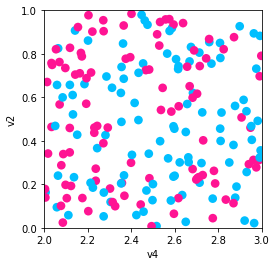
\includegraphics[width=\textwidth]{figures/code/scatter_0.png}
    \end{subfigure}
    \begin{subfigure}{0.5\textwidth}
        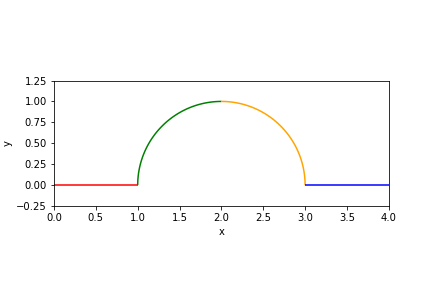
\includegraphics[width=\textwidth]{figures/code/line_1.png}
    \end{subfigure}
    \caption{Scatter plot and line plot implemented using prototype artists and data models, building on Matplotlib rendering.}
    \label{fig:code_scatter_line}
\end{figure}
To prototype our model, we implemented the artist classes for the scatter and line plots shown in figure~\ref{fig:code_scatter_line} because they differ in every attribute: different visual channels \vchannel\ that composite to different marks \vmark\ with different continuities \vindex\.  We make use of the Matplotlib figure and axes artists \cite{hunterArchitectureOpenSource,hunterMatplotlib2DGraphics2007} so that we can initially focus on the data to graphic transformations. 

To generate the images in figure~\ref{fig:code_scatter_line}, we instantiate \mintinline{python}{fig, ax} artists that will contain the new \mintinline{python}{Point, Line} primitive objects we implemented based on our topology model. 

\begin{multicols*}{2}
\begin{minted}{python}
    fig, ax = plt.subplots()
    artist = Point(data, transforms)
    ax.add_artist(artist)
\end{minted}
\columnbreak
\begin{minted}{python}
    fig, ax = plt.subplots()
    artist = Line(data, transforms)
    ax.add_artist(artist)
\end{minted}
\end{multicols*}

We then add the \mintinline{python}{Point} and \mintinline{python}{Line} artist that construct the scatter and line graphics. These artists are implemented as the equivalence class \vartisteq\ with the aesthetic configurations factored out into a \mintinline{python}{transforms} dictionary that specifies the visual bundle \vtotal\. The equivalence classes \vartisteq\ map well to Python classes since the functional aspects-\vchannel, \vmarkd, and \vindex - are completely reusable in a consistent composition, while the visual values in \vtotal\ are what change between different artists belonging to the same class \vartisteq. The \mintinline{python}{data} object is an abstraction of a data bundle \dtotal\ with a specified section \dsection. Implementing \gtotal\ and \gsection\ are out of scope for this prototype because they are part of the rendering process. We also did not implement any form of \vindex\ because the scatter, line, and bar plots prototyped here directly broadcast from \dbasepoint\ to \gbasepoint, unlike for example an image which may need to be rotated. 
 
\subsection{Artist Class $\vartist^{\prime}$}
\label{sec:code_artist}
The artist is the piece of the matplotlib architecture that constructs an internal representation of the graphic that the render then uses to draw the graphic. In the prototype artist, \mintinline{python}{transform} is a dictionary of the form \mintinline{python}|{parameter:(variable, encoder)}| where parameter is a component in \vfiber, variable is a component in \dfiber,  and the \vchannel\ encoders are passed in as functions or callable objects. The data bundle \dtotal\ is passed in as a \mintinline{python}{data} object. By binding data and transforms to \vartisteq\ inside \mintinline{python}{__init__}, the \mintinline{python}{draw} method is a fully specified artist \vartist.

\begin{minted}[escapeinsize=||]{python}
class ArtistClass(matplotlib.artist.Artist):
    |\label{code:artist}|
    def __init__(self, data, transforms, *args, **kwargs):
        # properties that are specific to the graphic but not the channels
        self.data = data 
        self.transforms = transforms
        super().__init__(*args, **kwargs)

    def assemble(self, **args):
        # set the properties of the graphic

    def draw(self, renderer):
        # returns K, indexed on fiber then key 
        # is passed the 
        view = self.data.view(self.axes) 
        # visual channel encoding applied fiberwise 
        visual = {p: t['encoder'](view[t['name']])
                  for p, t in self.transforms.items()}
        self.assemble(**visual)
        # pass configurations off to the renderer
        super().draw(renderer)
\end{minted}

The data is fetched in section \dsection\ via a \mintinline{python}{view} method on the data because the input to the artist is a section on \dtotal. The \mintinline{python}{view} method takes the \mintinline{python}{axes} attribute because it provides the region in graphic coordinates \gbase\ that we can use to query back into data to select a subset as discussed in section~\ref{sec:data_sheaf_stalk}. The \vchannel\ functions are then applied to the data to generate the visual section \vsection\ that here is the object \mintinline{python}{visual}. The conversion from data to visual space is simplified here to directly show that it is the encoding \vchannel\ applied to the component. In the full implementation, we allow for fixed visual parameter, such as setting a constant color for all sections, by verifying that the named component is in \dfiber\ before accessing the data. If the data component name is not in \dfiber\, this is interpreted to mean this component is a thickening of \vtotal that could be pulled back to \dtotal\ via an inverse identity \vchannel. 

The components of the visual object, denoted by the Python unpacking convention \mintinline{python}{**visual} are then passed into the \mintinline{python}{assembly} function that is \vmarkd. This assembly function is responsible for generating a representation of the glyph such that it could be serialized to recreate a static version of the graphic. Although \mintinline{python}{assemble} could be implemented outside the class such that it returns an object the artist could then parse to set attributes, the attributes are directly set here to reduce indirection. This artist is not optimized because we prioritized demonstrating the separability of \vchannel\ and \vmarkd. The last step in the artist function is handing itself off to the renderer. The extra \mintinline{python}{*arg, **kwargs} arguments in \mintinline{python}{__init__,draw} are artifacts of how these objects are currently implemnted in Matplotlib. 

The \mintinline{python}{Point} artist builds on \mintinline{python}{collection} artists because collections are optimized to efficiently draw a sequence of primitive point and area marks. In this prototype, the scatter marker shape is fixed as a circle, and the only visual fiber components are x and y position, size, and the facecolor of the marker. We only show the \mintinline{python}{assembly} function here because the \mintinline{python}{__init__, draw} are identical the prototype artist shown in \ref{code:artist}. 
\begin{minted}{python}
class Point(mcollections.Collection):
    def assemble(self, x, y, s, facecolors='C0' ):
        # construct geometries of the circle glyphs in visual coordinates
        self._paths = [mpath.Path.circle(center=(xi,yi), radius=si) 
                    for (xi, yi, si) in zip(x, y, s)] 
        # set attributes of glyphs, these are vectorized 
        # circles and facecolors are lists of the same size
        self.set_facecolors(facecolors)
\end{minted} 
The \mintinline{python}{view} method repackages the data as a fiber component indexed table of vertices, as described in section~\ref{sec:triangulization}. Even though the \mintinline{python}{view} is fiber indexed, each vertex at an index \dbasepoint has corresponding values in section $\dsection(\dbasepoint_{i})$. This means that all the data on one vertex maps to one glyph. To ensure the integrity of the section, \mintinline{python}{view} must be atomic. This means that the values cannot change after the method is called in draw until a new call in draw. We put this constraint on the return of the \mintinline{python}{view} method so that we do not risk race conditions. 

This table is converted to a table of visual variables and is then passed into \mintinline{python}{assemble}. In  \mintinline{python}{assemble}, the \vsection\ components are used to construct the vector path of each circular marker with center \texttt{(x,y)} and size \texttt{x} and set the colors of each circle. This is done via the \mintinline{python}{Path.circle} object. As mentioned in sections ~\ref{sec:data_sheaf_stalk} and \ref{sec:artist_q}, this assembly function could as easily be implemented such that it was fed one $\dsection(\dbasepoint)$ at a time. 

The main difference between the \mintinline{python}{Point} and \mintinline{python}{Line} objects is in the \mintinline{python}{assemble} function because line has different continuity from scatter and is represented by a different type of graphical mark. 

\begin{minted}{python}
class Line(mcollections.LineCollection):
    def assemble(self, x, y, color='C0'):
            #assemble line marks as set of segments 
            segments = [np.vstack((vx, vy)).T for vx, vy 
                        in zip(x, y)]
            self.set_segments(segments)
            self.set_color(color)
\end{minted}
In the \mintinline{python}{Line} artist, \mintinline{python}{view} returns a table of edges. Each edge consists of (x,y) points sampled along the line defined by the edge and information such as the color of the edge. As with \mintinline{python}{Point}, the data is then converted into visual variables. In \mintinline{python}{assemble}, this visual representation is composed into a set of line segments, where each segement is the array generated by \mintinline{python}{np.vstack((vx, vy))}. Then the colors of each line segment are set. The colors are guaranteed to correspond to the correct segment because of the atomicity constraint on view. 

\begin{figure}[H]
    \begin{subfigure}{0.5\textwidth}
        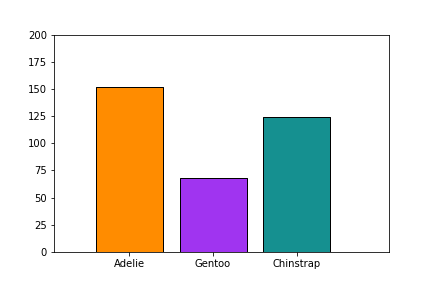
\includegraphics[width=\textwidth]{figures/code/bar_v.png}
    \end{subfigure}
    \begin{subfigure}{0.5\textwidth}
        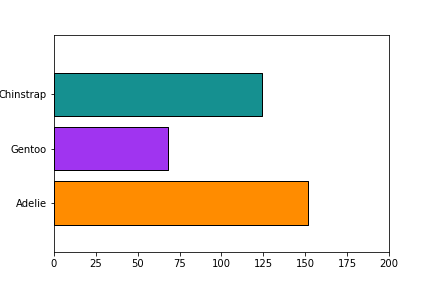
\includegraphics[width=\textwidth]{figures/code/bar_h.png}
    \end{subfigure}
    \caption{Frequency of Penguin types visualized as discrete bars. }
    \label{fig:code_bar_simple}
\end{figure}
The bar charts in figure~\ref{fig:code_bar_simple} are generated with a \mintinline{python}{Bar} artist. The have the same required \vfiber\ components of (position, length), but in \mintinline{pyton}{__init__} of \mintinline{python}{Bar} an additional parameter is set, \texttt{orientation} which controls whether the bars are arranged vertically or horizontally. This parameter only applies holistically to the graphic and never to individual data parameters, and highlights how the model encourages explicit differentiation between parameters in \vtotal\ and graphic parameters applied directly to \vmarkd\. 

\begin{minted}{python}
class Bar(mcollections.Collection):
    def __init__(self, data, transforms, orientation='v', *args, **kwargs):
        """
        orientation: str, optional
            v: bars aligned along x axis, heights on y
            h: bars aligned along y axis, heights on x
        """
        self.orientation = orientation
        super().__init__(*args, **kwargs)
        self.data = data
        self.transforms = copy.deepcopy(transforms)

    def assemble(self, position, length, floor=0, width=0.8, facecolors='C0', edgecolors='k', offset=0):
        #set some defaults
        width = itertools.repeat(width) if np.isscalar(width) else width
        floor = itertools.repeat(floor) if np.isscalar(floor) else (floor)
        
        # offset is passed through via assemblers such as multigroup, not supposed to be directly tagged to position 
        position = position + offset
        
        def make_bars(xval, xoff, yval, yoff):
             return [[(x, y), (x, y+yo), (x+xo, y+yo), (x+xo, y), (x, y)] 
                for (x, xo, y, yo) in zip(xval, xoff, yval, yoff)]
        #build bar glyphs based on graphic parameter
        if self.orientation in {'vertical', 'v'}:
            verts = make_bars(position, width, floor, length)
        elif self.orientation in {'horizontal', 'h'}:
            verts = make_bars(floor, length, position, width)
        
        self._paths = [mpath.Path(xy, closed=True) for xy in verts]
        self.set_edgecolors(edgecolors)
        self.set_facecolors(facecolors)
        
    def draw(self, renderer,  *args, **kwargs):
        view = self.data.view(self.axes)
        visual = {}
        for (p, t) in self.transforms.items():
            if isinstance(t, dict):
                if t['name'] in self.data.FB.F and 'encoder' in t:
                    visual[p] = t['encoder'](view[t['name']])
                elif 'encoder' in t: # constant value
                    visual[p] = t['encoder'](t['name'])
                elif t['name'] in self.data.FB.F: # identity 
                    visual[p] = view[t['name']]
            else: # no transform 
                 visual[p] = t
        self.assemble(**visual)
        super().draw(renderer,  *args, **kwargs)
    
\end{minted}
The \mintinline{python}{draw} method here has a more complex unpacking of visual encodings to support passing in visual component data directly. This is vastly simplifies building composite objects as the alternative would be higher order functions that take as input the transforms passed in by the user. This construction supports a constant visual parameter, an identity transform where the value is the same in \dtotal\ and \vtotal\, and setting the visual component directly. The \mintinline{python}{assemble} function constructs bars and sets their face and edge colors. The \mintinline{python}{make_bars} function converts the input position and length to the coordinates of a rectangle of the given width. Defaults are provided for 'width' and 'floor' to make this function more reusable. Typically the defaults are used for the type of chart shown in figure~\ref{fig:code_bar_simple}, but these visual variables are often set when building composite versions of this chart type as discussed in section~\ref{sec:code_case_study}. 


\subsection{Encoders \vchannel}
\label{sec:code_channels}
As mentioned above, the encoding dictionary is specified by the visual fiber component, the corresponding data fiber component, and the mapping function. The visual parameter serves as the dictionary key because the visual representation is constructed from the encoding applied to the data  $\vsection = \vchannel \circ \dsection$. For the scatter plot, the mappings for the visual fiber components $\vfiber=(x,y, facecolors, s)$ are defined as
\begin{minted}{python}
cmap =  color.Categorical({'true':'deeppink', 'false':'deepskyblue'})
transforms = {'x': {'name': 'v4', 'encoder': lambda x: x},
              'y': {'name': 'v2', 'encoder': lambda x: x},
              'facecolors': {'name':'v3', 'encoder': cmap}, 
              's':{'name': None , 'encoder': lambda _: itertools.repeat(.02)}}
\end{minted}
where the position \textit{(x,y)} \vchannel\ transformers are identity functions. The size \textit{s} transformer is not acting on a component of \dfiber, instead it is a \vchannel\ that returns a constant value. While size could be embedded inside the \mintinline{python}{assembly} function, it is added to the transformers to illustrate user configured visual parameters that could either be constant or mapped to a component in \dfiber. The identity and constant \vchannel\ are explicitly implemented here to demonstrate their implicit role in the visual pipeline, but they are somewhat optimized away in \mintinline{python}{Bar}. More complex encoders can be implemented as callable classes, such as 
\begin{minted}{python}
class Categorical:
    def __init__(self, mapping):
        # check that the conversion is to valid colors
        assert(mcolors.is_color_like(color) for color in mapping.values())
        self._mapping = mapping

    def __call__(self, value):
        # convert value to a color
        return [mcolors.to_rgba(self._mapping[v]) for v in values]
\end{minted}

where \mintinline{python}{__init__} can validate that the output of the \vchannel\ is a valid element of the \vfiber\ component the \vchannel\ function is targeting. Creating a callable class also provides a simple way to swap out the specific (data, value) mapping without having to reimplement the validation or conversion logic. A test for equivariance can be implemented trivially
\begin{minted}{python}
def test_nominal(values, encoder):
    m1 = list(zip(values, encoder(values)))
    random.shuffle(values)
    m2 = list(zip(values, encoder(values)))
    assert sorted(m1) == sorted(m2)
\end{minted}
but is currently factored out of the artist for clarity. In this example, \mintinline{python}{is_nominal} checks for equivariance of permutation group actions by applying the encoder to a set of values, shuffling values, and checking that (value, encoding) pairs remain the same.

\subsection{Data \dtotal}
\label{sec:code_data}
The data input into the \mintinline{pythin}{Artist} will often be a wrapper class around an existing data structure. This wrapper object must specify the fiber components \dfiber\ and connectivity \dbase\ and have a \mintinline{view} method that returns an atomic object that encapsulates \dsection\. The object returned by the view must be key valued pairs of \mintinline{python}|{component name : component section}| where each section is a component as defined in equation~\ref{eq:data_section_decompose}. To support specifying the fiber bundle, we define a \mintinline{python}{FiberBundle} data class\cite{DataclassesDataClasses}

\begin{minted}{python}
@dataclass
class FiberBundle:
"""
Attributes
----------
K: {'tables': []}
F: {variable name: {'type': type, 'moniod', 'range': []}}
"""
    K: dict 
    F: dict
\end{minted}

that asks the user to specify how \dbase is triangulated and the attributes of \dfiber. Python dataclasses are a good abstraction for the fiber bundle class because the \mintinline{python}{FiberBundle} class only stores data. The \dbase\ is specified as tables because the \mintinline{python}{assembly} functions expect tables that match the continuity of the graphic; scatter expects a vertex table because it is discontinuous, line expects an edge table because it is 1D continuous. The fiber informs appropriate choice of \vchannel\, therefore it is a dictionary of attributes of the fiber components. 

To generate the scatter plot in figure~\ref{fig:code_scatter_line}, we fully specify a dataset with random keys and values in a section chosen at random form the corresponding fiber component. The fiberbundle \mintinline{python}{FB} is a class level attribute since all instances of \mintinline{python}{code}{VertexSimplex} come from the same fiberbundle.
\begin{minted}{python}
class VertexSimplex: #maybe change name to something else
    """Fiberbundle is consistent across all sections
    """
    FB = FiberBundle({'tables': ['vertex']},  
            {'v1': {'type': float,'monoid':'interval','range': [0,1]},
             'v2': {'type': str, 'monoid':'nominal', 'range':['true', 'false']},
             'v3': {'type': float, 'monoid':'interval', 'range':[2,3]}})

    def __init__(self, sid = 45, size=1000, max_key=10**10):
        # create random list of keys
    def tau(self, k):
        # e1 is sampled from F1, e2 from F2, etc...
        return (k, (e1, e2, e3, e4))

    def view(self, axes):
        table = defaultdict(list)
        for k in self.keys:
            table['index'] = k
            # on each iteration, add one (name, value) pair per component
            for (name, value) in zip(self.FB.fiber.keys(), self.tau(k)[1]):
                table[name].append(value)
        return table
\end{minted}
The view method returns a dictionary where the key is a fiber component name and the value is a list of values in the fiber component. The table is built one call to the section method \mintinline{python}{tau} at a time, guaranteeing that all the fiber component values are over the same \dbasepoint. Table has a \mintinline{python}{get} method as it is a method on Python dictionaries. In contrast, the line in \mintinline{python}{EdgeSimplex} is defined as the functions \mintinline{python}{_color,_xy} on each edge. 

\begin{minted}{python}
class EdgeSimplex: 
    # assign a class level FB attribute
    def __init__(self, num_edges=4, num_samples=1000): 
        self.keys = range(num_edge) #edge id
        # distance along edge
        self.distances = np.linspace(0,1, num_samples)
        # half generlized representation of arcs on a circle
        self.angle_samples = np.linspace(0, 2*np.pi, len(self.keys)+1)

    @staticmethod
    def _color(edge):
        colors = ['red','orange', 'green','blue']
        return colors[edge%len(colors)]

    @staticmethod
    def _xy(edge, distances, start=0, end=2*np.pi):
        # start and end are parameterizations b/c really there is 
        angles = (distances *(end-start)) + start
        return np.cos(angles), np.sin(angles)

    def tau(self, k): #will fix location on page on revision
        x, y = self._xy(k, self.distances, 
                        self.angle_samples[k], self.angle_samples[k+1]) 
        color = self._color(k) 
        return (k, (x, y, color))

    def view(self, axes):
        table = defaultdict(list)
        for k in self.keys:
            table['index'].append(k)
            # (name, value) pair, value is [x0, ..., xn] for x, y
            for (name, value) in zip(self.FB.fiber.keys(), self.tau(k, simplex)[1]):
                table[name].append(value)
\end{minted}
Unlike scatter, the line section method \mintinline{python}{tau} returns the functions on the edge evaluated on the interval [0,1]. By default these means each \mintinline{python}{tau} returns a list of 1000 x and y points and the associated color. As with scatter, \mintinline{python}{view} builds a table by calling \mintinline{python}{tau} for each \dbasepoint\. Unlike scatter, the line table is a list where each item contains a list of points. This bookkeeping of which data is on an edge is used by the \mintinline{python}{assembly} functions to bind segments to their visual properties. 

\begin{figure}[H]
    \begin{subfigure}{0.5\textwidth}
        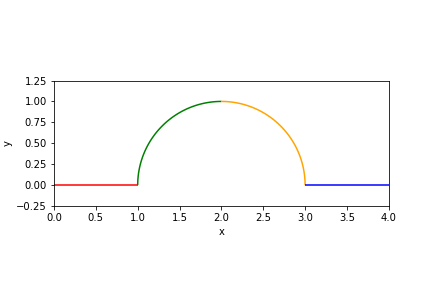
\includegraphics[width=\textwidth]{figures/code/linec_1.png}
    \end{subfigure}
    \begin{subfigure}{0.5\textwidth}
        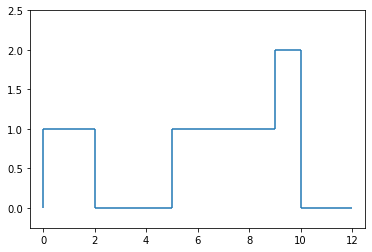
\includegraphics[width=\textwidth]{figures/code/lined_1.png}
    \end{subfigure}
    \caption{Continuous and discontinuous lines as defined by different data models, but generated with the same \vartisteq=\mintinline{python}{artist}}
    \label{fig:circle_step}
\end{figure}

The graphics in figure~\ref{fig:circle_step} are made using the \mintinline{python}{Line} artist and the \mintinline{python}{Graphline} data source

\begin{minted}{python}
class GraphLine:
    def __init__(self, FB, edge_table, vertex_table, num_samples=1000, connect=False):
        #s set args as attributes and generate distance
        if connect: # test connectivity if edges are continuous
            assert edge_table.keys() == self.FB.F.keys()
            assert is_continuous(vertex_table)

    def tau(self, k):
        # evaluates functions defined in edge table
        return(k, (self.edges[c][k](self.distances) for c in self.FB.F.keys()))

    def view(self, axes):
        """walk the edge_vertex table to return the edge function
        """
        table = defaultdict(list)
        #sort since intervals lie along number line and are ordered pair neighbors
        for (i, (start, end)) in sorted(zip(self.ids, self.vertices), key=lambda v:v[1][0]):
            table['index'].append(i)
            # same as view for line, returns nested list
            for (name, value) in zip(self.FB.F.keys(), self.tau(i, simplex)[1]):
                table[name].append(value)
        return table
\end{minted}
where if told that the data is connected, the data source will check for that connectivity by constructing an adjacency matrix. The multicolored line is a connected graph of edges with each edge function evaluated on 1000 samples 
\begin{minted}{python}
simplex.GraphLine(FB, edge_table, vertex_table, connect=True)
\end{minted}
while the stair chart is discontinuous and only needs to be evaluated at the edges of the interval 
\begin{minted}{python}
simplex.GraphLine(FB, edge_table, vertex_table, num_samples=2, connect=False)
\end{minted}
such that one advantage of this model is it helps differentiate graphics that have different artists from graphics that have the same artist but make different assumptions about the source data. 


\subsection{Case Study: Penguins}
For this case study, we use the Palmer Penguins dataset\cite{gormanEcologicalSexualDimorphism2014, horstPalmerpenguinsPalmerArchipelago2020} since it is multivariate and has a varying number of penguins. We use a version of the data packaged as a pandas dataframe\cite{nakhaeeMcnakhaeePalmerpenguins2021} since that is a very commonly used Python labeled data structure. The wrapper is very thin because there is explicitly only one section.
\begin{minted}{python}
class DataFrame:
    def __init__(self, dataframe):
        self.FB = FiberBundle(K = {'tables':['vertex']},
                              F = dict(dataframe.dtypes))
        self._tau = dataframe.iloc
        self._view = dataframe

    def view(self, axes=None):
        return self._view
\end{minted}
Since the aim for this wrapper is to be very generic, here the fiber is set by querying the dataframe for its metadata. The \mintinline{python}{dtypes} are a list of column names and the datatype of the values in each column; this is the minimal amount of information the model requires to verify constraints. The pandas indexer is a key valued set of discrete vertices, so there is no need to repackage for the data interface. 

\begin{figure}[H]
    \begin{subfigure}{0.5\textwidth}
        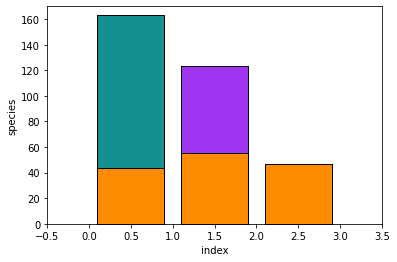
\includegraphics[width=\textwidth]{figures/code/bar_stacked.png}
    \end{subfigure}
    \begin{subfigure}{0.5\textwidth}
        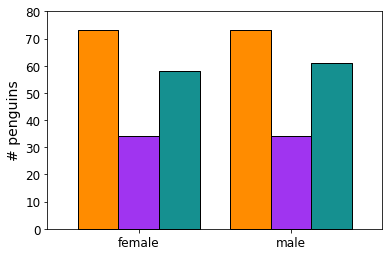
\includegraphics[width=\textwidth]{figures/code/bar_grouped.png}
    \end{subfigure}
    \caption{Penguin count disaggregated by island and species}
    \label{fig:code_bar_multi}
\end{figure}

The stacked and grouped bar charts in figure~\ref{fig:code_bar_multi} are both out of \mintinline{python}{Bar} artists such that the difference between \mintinline{Python}{StackedBar} and \mintinline{Python}{GroupedBar} is specific to the ways in which the \mintinline{python}{Bar} are arranged differently. These two artists have identical \mintinline{{python}{__init__} and \mintinline{python}{draw} methods. As with \mintinline{python}{Bar}, the orientation is set on instantiation. In both these artists, we separate the transforms applied to only one component \mintinline{python}{transforms} and the case \mintinline{python}{mtransforms} where the same transform is applied to multiple components such that \votal\ has multiple components that map to the same retinal variable. 
\begin{minted}{python}
class StackedBar(martist.Artist):
    def __init__(self, data, transforms, mtransforms, orientation='v', *args, **kwargs):
        """
        Parameters
        ----------
   
        orientation: str, optional
            vertical: bars aligned along x axis, heights on y
            horizontal: bars aligned along y axis, heights on x   
        """
        super().__init__(*args, **kwargs)
        self.data = data
        self.orientation = orientation
        self.transforms = copy.deepcopy(transforms)
        self.mtransforms = copy.deepcopy(mtransforms)

    def assemble(self):
        view = self.data.view(self.axes)
        self.children = [] # list of bars to be rendered
        floor = 0
        for group in self.mtransforms:
            # pull out the specific group transforms
            group['floor'] = floor
            group.update(self.transforms)
            bar = Bar(self.data, group, self.orientation, transform=self.axes.transData)
            self.children.append(bar)
            floor += view[group['length']['name']]
            
            
    def draw(self, renderer, *args, **kwargs):
        # all the visual conversion gets pushed to child artists
        self.assemble()
        #self._transform = self.children[0].get_transform()
        for artist in self.children:
            artist.draw(renderer, *args, **kwargs)

\end{minted}
Since all the visual transformation is passed through to \mintinline{python}{Bar}, the \mintinline{python}{draw} method does not do any visual transformations. In \mintinline{Python}{StackedBar} the \mintinline{python}{view} is used to adjust the \mintinline{python}{floor} for every subsequent bar chart since a stacked bar chart is bar chart area marks concatenated together in the length parameter. In contrast, \mintinline{Python}{GroupedBar} does not even need the view, but instead keeps track of the relative position of each group of bars in the visual only variable \mintinline{python}{offset}. 

\begin{minted}{python}
class GroupedBar(martist.Artist):
    def assemble(self):
        self.children = [] # list of bars to be rendered
        ngroups = len(self.mtransforms)
        
        for gid, group in enumerate(self.mtransforms):
            group.update(self.transforms)
            width = group.get('width', .8)
            group['width'] = width/ngroups
            group['offset'] = gid/ngroups*width 
            bar = Bar(self.data, group, self.orientation, transform=self.axes.transData)     
            self.children.append(bar)
\end{minted}{python}

Since the only difference between these two glyphs is in the composition of \mintinline{python}{Bar}, they take in the exact same transform specification dictionaries. \mintinline{python}{transform} dictates the position of the group, in this case by island the penguins are found on.

\begin{minted}{python}
transforms = {'position': {'name':'island',
              'encoder': position.Nominal({'Biscoe':0.1, 'Dream':1.1, 'Torgersen':2.1})}} 
group_transforms =  [{'length': {'name':'Adelie'},
                      'facecolors': {'name':"Adelie_s", 'encoder':cmap}},
                     {'length': {'name':'Chinstrap'},
                      'facecolors': {'name':"Chinstrap_s", 'encoder':cmap}}, 
                     {'length': {'name':'Gentoo'},
                      'facecolors': {'name':"Gentoo_s", 'encoder':cmap}}]
\end{minted}
\mintinline{python}{group_transforms} describes the group, and takes a list of dictionaries where each dictionary is the aesthetics of each group. That \mintinline{python}{position} and \mintinline{python}{length} are required parameters is enforced in the creation of the \mintinline{python}{Bar} artist. These means that these two artists have identical function signatures

\begin{minted}{python}
artistSB = bar.StackedBar(bt, ts, group_transforms)
artistGB = bar.GroupedBar(bt, ts, group_transforms)
\end{minted}

but differ in assembly \vmarkd. By decomposing the architecture into data, visual encoding, and assembly steps, we are able to build components that are more flexible and also more self contained than the existing code base. While very rough, this API demonstrates that the ideas presented in the math framework are implementable. In choosing a functional approach, if not implementation, we provide a framework for library developers to build reusable encoder \vchannel\, assembly \vmarkd and artists \vartist. We argue that  if these functions are built such that they are equivariant with respect to monoid actions and the graphic topology is a deformation retraction of the data topology, then the artist by definition will be a structure and property preserving map from data to graphic. 
\end{document}